\chapter{多样化Handler虚拟机加壳的研究与实现}

在软件反逆向工程中的虚拟机和虚拟机模拟软件是完全不同的东西,本章描述的虚拟机保护方法是类似于一种解释执行系统,它和解释型语言如Python、Lua、Ruby等有相似的地方。

%本节会对虚拟机加壳方案进行设计,并且详细叙述加密过程和解密过程,如图\ref{cha2:fig:addshell}所示
对于PE文件结构,在\ref{cha2:sec:PEfile}节有详细的分析结果,对于虚拟机加壳比较重要的位置是节表Section Table,原始PE程序的二进制硬编码通常是按照顺序排列在多个节表中的,在通过分析PE文件的DOS Header和PE Header后,可以通过里面的相关信息,计算出Section Table的起始偏移地址,得到代码区域的地址后,将此部分标记为待保护汇编的指令流的起始区域,由次区域开始到下一个.rdata节截止,对原始PE程序的二进制硬编码进行加密保护。

%\begin{figure}[h] 
%	\centering
%	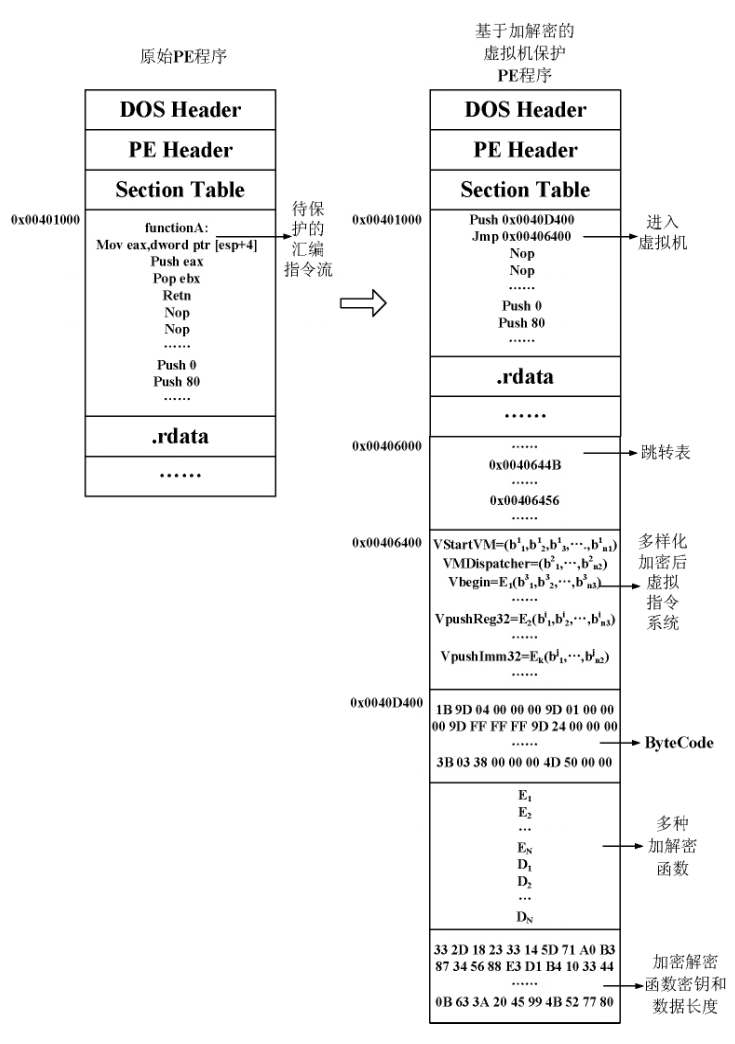
\includegraphics[height=18cm]{addshell.png}
%	\caption{虚拟机加壳过程}
%	\label{cha2:fig:addshell}
%\end{figure}


本章节将会设计一个在PE程序中的虚拟机壳,程序的OEP(Original Entry Point)程序的入口点将会被改变为虚拟机的入口点,进行虚拟机的执行区域。虚拟机将会进行一系列的初始化工作:对原有的汇编代码进行整理、提取出其中的导入表信息、建立Handler等。建立调度器dispatcher,调度器会将原本的寄存器符号统统压入栈中,把esi指向虚拟机字节码的起始地址,ebp指向当前的真实栈区域,edi指向VMContext虚拟环境结构,在执行上述过程后,虚拟机初始化环境将会加载完毕。



\section{虚拟机保护方法基本原理}


首先虚拟机保护系统会将可执行程序反汇编为CUP可以理解的X86指令流,做出一套X86指令和字节码之间的映射,再讲X86指令流的汇编代码转换为字节码,此时可执行程序已经完成了压缩阶段。最后,虚拟机保护会系统会将解释器内嵌到可执行程序中,使得被保护的代码在程序执行时可以被正确翻译后执行,整个流程类似于Java的虚拟机。

具体保护步骤如下:

Step1 将带保护程序使用反汇编引擎转换为汇编指令;

Step2 将汇编指令转换为一对一的字节码;

Step3 建立Handler表和跳转表;

Step4 将上述三个步骤产生的文件打包为可执行文件,使用虚拟环境结构VMContext存储寄存器中的值,将字节码、虚拟环境结、Handlers、Dispather打包为一个新节,并添加到可执行程序中,虚拟机代码保护机制的流程如图\ref{codeprotect}所示 。
\begin{figure}[htbp]
	\centering
	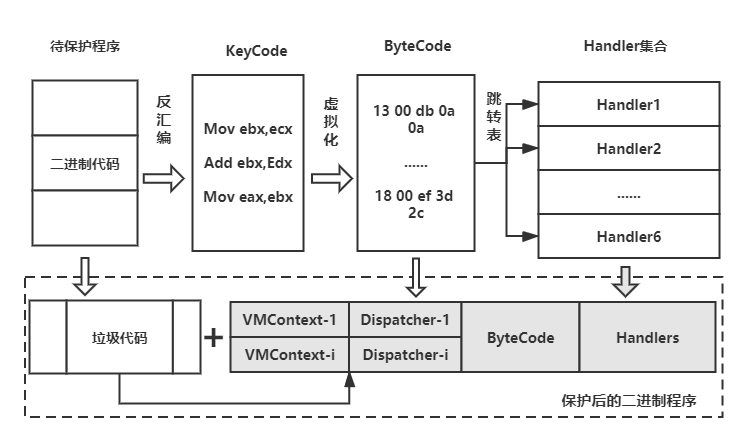
\includegraphics[width=14cm]{codeprotect.png}
	\bicaption{虚拟机代码保护机制}{Virtual machine code protection mechanism}
	\label{codeprotect}
\end{figure}

\subsection{相关反汇编工具}

反汇编器是把高级语言写成的程序翻译成汇编语言的工具,反汇编程序的目标是高级语言如C/C++、VB,而不是汇编语言,它通常输出为了便于阅读而不是适合汇编程序输入而设置的格式,反汇编器会给阅读反汇编代码者提供大量的可参考数据\cite{张泉2018Win32}。

本课题采用的是OllyDbg引擎提供的开源反汇编器,在进行反汇编过程中,它可以自动跟踪寄存器、识别函数、API调用,给阅读者带来很大的方便,由于其易用性和可用性,此软件在分析恶意代码时也很有用\cite{乐德广2018一种抵御逆向工程的安卓应用混淆技术研究}。

\subsection{X86指令}

按照x86体系结构,按照功能分为流指令、普通指令、栈指令、和不可模拟指令4类\cite{曹宏盛2019一种用于}。

流指令是指跳转指令、函数调用指令、返回指令等改变文件执行流程的指令。

普通指令指add、sub、mov等加减运算和数据传输指令。

栈指令指压栈指令弹出栈指令等操作栈空间的指令。

不可模拟指令指无法被模拟的指令,这类指令通常硬件相关,比如int3、in、out等指令。

指令分类如表\ref{registers}所示。

\begin{table}[htbp]
	\bicaption{X86汇编指令分类}{X86 assembly instruction classification}
	\label{registers}
	\begin{tabular}{l|l|l|l|l|l}
		\hline
		\multicolumn{2}{c|}{无操作数指令} & 单操作数指令 & \multicolumn{2}{l|}{双操作数指令} & 多操作数指令 \\ \hline
		AAA          & STC           & CALL   & ADC         & XADD          & IMUL   \\ \hline
		AAD          & STD           & JMP    & ADD         & XCHG          & SHLD   \\ \hline
		AAM          & STI           & JCC    & AND         & CMP           & SHRD   \\ \hline
		AAS          & INSB          & LOOP   & MOV         & CMPS          & -      \\ \hline
		CBW          & INSW          & LOOPE  & OR          & LEA           & -      \\ \hline
		CDQ          & INSD          & LOOPNE & RCL         & MOVSX         & -      \\ \hline
		CLD          & LAHF          & INC    & RCR         & MOVZX         & -      \\ \hline
		CLI          & LODSB         & DEC    & ROL         & -             & -      \\ \hline
	\end{tabular}
	\centering

\end{table}

基于虚拟机Handler动态加密的情况大致如图\ref{virtual}所示。其中VStartVM部分初始化虚拟机,VMDispatcher调度每一个Handler。在程序运行时,字节码就是操作系统需要识别的二进制代码,VMregisters就是操作系统的调度器,不同的Handler对应不同的汇编代码,相对应的就是机器码。

\begin{figure}[htbp]
	 
	\centering
	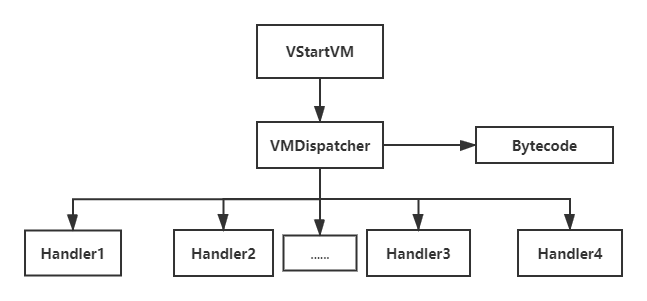
\includegraphics[height=6cm]{virtual.png}
	\bicaption{虚拟机执行时的情况}{When the virtual machine executes}
	\label{virtual}
\end{figure}



\section{调用约定和框架}

\subsection{虚拟环境}
\label{cha3:sec:virtualcontext}
解释器在执行时识别的是字节码,所以需要使用一个结构来保存CPU中寄存器的值,其结构设计具体如图\ref{context}所示\cite{胡浔惠2019一种应用随机森林的代码混淆路径分支技术}。

\begin{figure}[htbp]
	
	\centering
	
	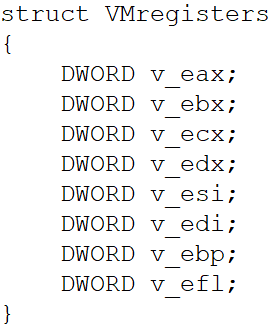
\includegraphics[height=5cm]{symbol.png}
	\bicaption{虚拟环境结构}{Virtual environment structure}
	\label{context}
\end{figure}

使用VMregisters结构体来存储eax,ebx等重要的寄存器,需要注意的是,这个结构体中不需要存放esp这个寄存器的,esp一直指向栈顶,而程序的执行本身需要栈空间的,esp寄存器的值就是ebp寄存器的值。

\subsection{调度器}

MbeginVM将原程序的环境中大部分寄存器的值压栈之后会建立一个VMDispatcher标签,Handler会循环执行这部分代码,如图\ref{begin}所示的代码MbeginVM部分也称为调度器。

\begin{figure}[htbp]
	\centering
	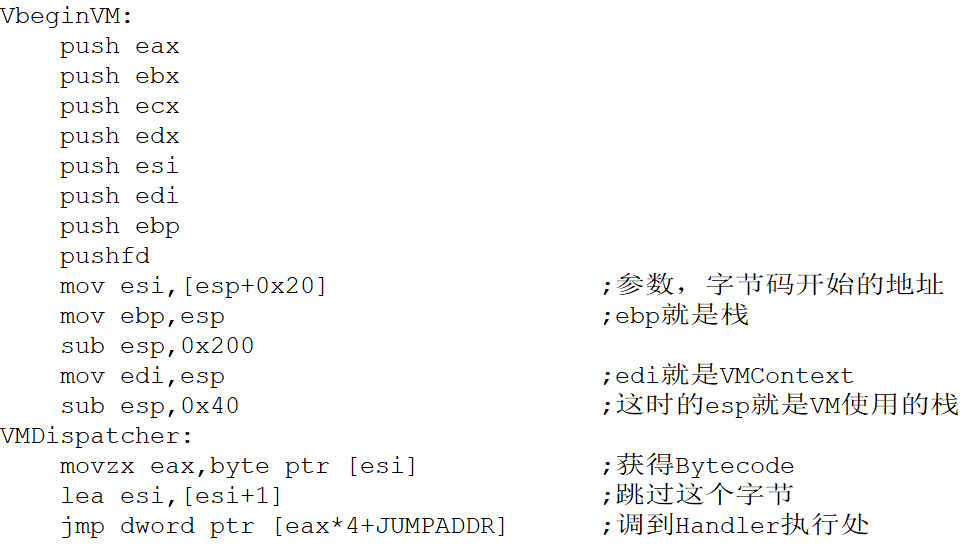
\includegraphics[height=8cm]{begin.png}
	\bicaption{Handler核心执行代码}{The Handler core executes the code}
	\label{begin}
\end{figure}


首先,调度器会将所有的CPU寄存器压栈,esi是设计的字节码的开始地址,ebg是原程序的栈空间,edi是虚拟环境结构,esp减去50h(不固定)就是虚拟机使用的栈空间地址。将虚拟机的虚拟环境结构和栈空间都放在了当前栈的300h处。

由于栈空间是变化的,这块区域可能在执行时被使用栈空间的语句覆盖,所以要设定一个机制保护本区域,当虚拟机在执行有关栈空间的指令时,需要有代码检查使用的空间是否覆盖到这块存放的数据,如果覆盖,则将这块结构向下移动。从“movze eax,byte ptr[esi]”指令开始读字节码。读取一个字节,就到跳转表中找到相应的Handler并执行相关语句。

这里会产生三个寄存器和某些值一直是对应关系,edi始终和虚拟环境结构的值相同,esi是当前字节码的地址,ebp一直是真实栈的地址。这三个对应关系在整个虚拟机执行过程中是一直成立的。通常情况下,这三个寄存器只能用作上述三个功能,不能使用做其他用途,如果必须使用则需要使用pushad来保护起所有的寄存器,在使用后需要使用popad恢复所有寄存器的值。


\section{多样化Handler设计}

本文所说Handler与Windows中的句柄Handler不同,本文的Handler指把某一段代码表示的功能给包装起来,形成可重复使用的功能结构块,它通常是被虚拟机保护中的调度器使用。Handler结构是虚拟机保护系统的核心部分,通常也是逆向攻击者的重点攻击对象,Handler结构中存放着字节码和汇编代码之间的转化过程,虽然可能这个转化过程不是通过一个Handler实现的,可能是由多个有着不同功能的Handler共同实现的,但是保护Handler等于保护了核心的翻译模块。所以,对Handler进行保护显得尤为重要,本节将会描述一种通过设计多样化的Handler使得逆向攻击者难以逆向分析字节码转化为汇编代码之间的翻译过程。

\subsection{辅助和普通Handler的实现}

Handler根据指令功能的不同可以分为两大类:一类是辅助Handler,通常存放着维护栈帧结构、CPU寄存器、堆结构等比较重要的Handler。另一类是普通Handler,通常存储着算术指令和跳转等基础指令。

\subsubsection{辅助Handler}
辅助Handler的示例代码如图\ref{fuzhu}所示,实现了PUSH寄存器指令、PUSH标志位指令、POP寄存器指令。

\begin{figure}[htbp]
	\centering
	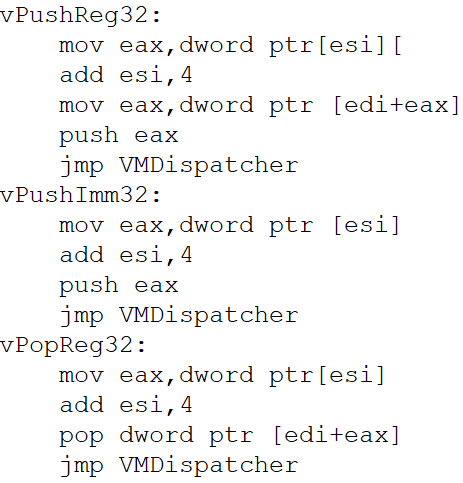
\includegraphics[height=7cm]{fuzhu.png}
	\bicaption{辅助Handler执行核心代码}{The helper Handler executes the core code}
	\label{fuzhu}
\end{figure}

\subsubsection{普通Handler}

\label{normalhandler}
在图\ref{fuzhu}的基础上,可以实现普通指令Handler,其实现代码如图\ref{normal}所示。

\begin{figure}[htbp]
	\centering
	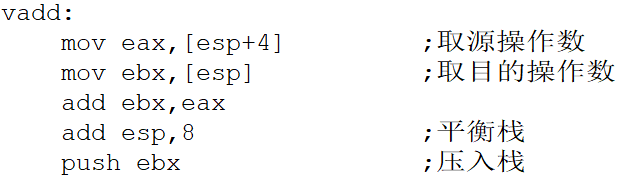
\includegraphics[height=2.5cm]{normal.png}
	\bicaption{普通Handler执行核心代码}{The normal Handler executes core code}
	\label{normal}
\end{figure}


将一个普通的汇编指令分为两个部分进行,指令的实现由普通Handler处理,目的操作数和源操作数都交由栈Handler处理。这样可以用更少的模拟Handler实现真正的汇编指令。

举一个例子便于理解。例如,sub指令的形式通常有“sub reg,imm”,“sub reg,reg”,“sub mem,reg”等,这里采用现将两个操作数使用栈Handler处理,将两个操作数存放在栈中,然后再调用“vsub Handler”,在这时两个操作数已经以立即数的形式在栈中,则“vsub Handler”可以直接默认栈顶就存放着它需要处理的数据,接着可以直接对栈顶这两个立即数进行减操作。
%vsubHandler的汇编代码如下。

%图

%再给出两个转换过程的伪代码,如下

%sub命令转化

%图1 图2 
%p744

%

\subsection{多样化Hanlder实现}

本课题的核心保护模块则是使用了多样化Handler模块,所谓多样化,就是将同一个Handler功能的模块采用多种设计方案,比如转移指令、算术指令、CALL指令等,由于汇编语言的特性,往往相同的功能可以采用多用方式实现,一旦相同功能采用不同汇编代码实现,逆向攻击者在分析虚拟机时会得到不同的Handler结果,并且每次分析的结果可能都不一样,使得逆向攻击者不能获得正确的Handler,也就无法掌握由汇编代码到字节码的翻译过程,通过这种方式,可以有效加大逆向攻击者的逆向分析难度。

\subsubsection{转移指令多样化}

转移指令一共包括四种指令,分别是无条件转移、条件转移、CALL和RETN。

由于无条件转移在汇编语句中就是JMP指令,而JMP指令的核心实现就是改变寄存器EIP的值无条件跳转指令JMP的Handler比较简单,如图\ref{jmpzhiling}所示。

\begin{figure}[htbp]
	\centering
	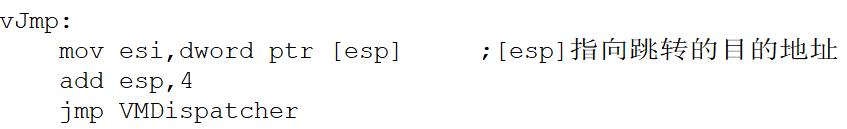
\includegraphics[width=13cm]{jmpzhiling.png}
	\bicaption{jmp的Handler实现代码}{The Handler implementation code for JMP}
	\label{jmpzhiling}
\end{figure}


JMP指令的功能太过单一,多样化的实现意义不大,所以本节将会介绍条件转移的多样化方法。X86的条件转移指令和条件传输指令是可以通过某种方式对应起来的,其比较如表\ref{jmp}所示。

\begin{table}[htbp]
	\bicaption{条件转移指令和条件传输指令}{Conditional transfer instruction and conditional transfer instruction}
	\begin{tabular}{c|c}
		
		\hline
		条件转移指令 & 条件传输指令 \\ \hline
		jne    & cmovne \\ \hline
		ja     & cmova  \\ \hline
		jb     & comvae \\ \hline
		jbe    & comvbe \\ \hline
		je     & comve  \\ \hline
		jg     & comvg  \\ \hline
	\end{tabular}
	\centering

	\label{jmp}
\end{table}
所有条件跳转指令都有对应的条件传输指令,图\ref{jne}是通过设计之后,条件跳转指令和条件传输指令的实现方法。

\begin{figure}[htbp]
	\centering
	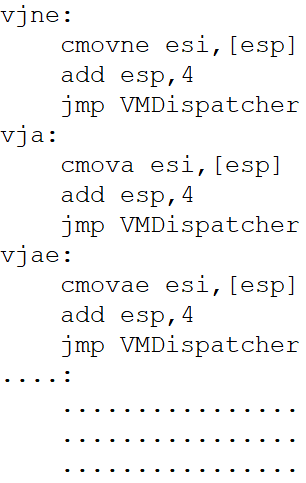
\includegraphics[width=5cm]{jne.png}
	\bicaption{条件跳转指令的另一种实现}{Another implementation of conditional jump instruction}
	\label{jne}
\end{figure}


这里再提出一种方式实现转移指令多样化,可以使用X86平台下的标志寄存器和无条件转移指令实现另一种跳转命令模拟跳转,原理是条件转移命令本身就是判断标志寄存器中的值实现跳转的,而存在其他指令可以直接读取标志寄存器的值,直接判断标志寄存器中的值,加上无条件跳转JMP的配合,就可以实现条件跳转。

%这里以JAE指令为例,代码如下。

%图746

%下图是伪代码的调用。

%vPush jmpto add adfa 
%d
%sdf
%adfa
%sdf

%上述过程为,首先读取标志位,根据取得的值(CF位)和1做and运算。使用CMOVE指令判断ZF标志位是否为0,如果为0就改变ESI的值。JAE指令只判断CF位。

%再举一个JBE指令的例子,Handler的汇编代码如下。

%图

%通过JAE指令和JBE指令的举例,实现了同一个Handler指令的多种实现方式,其他条件跳转指令转化原理基本一致,这里不再举例。

\subsubsection{算术指令多样化}


在X86指令体系中存在一些不同指令可以用同一种指令去实现的情况,它们的目的都是将esi指令加一,但是却是inc指令和add指令的不同实现方式,示例代码图\ref{add}所示。


\begin{figure}[htbp]
	\centering
	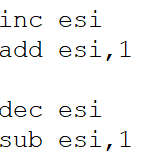
\includegraphics[width=2.3cm]{add.png}
	\bicaption{add指令和sub指令的另一种形式}{Another form of the Add and SUB directives}
	\label{add}
\end{figure}


X86体系中存在很多这种指令,实现原理于图\ref{add}类似,在Handler多样化实现时都可以利用这种机制,实现汇编到字节码翻译过程中的Hanlder指令多样化。

具体操作方式则是如\ref{normalhandler}节所述,将操作指令、目的操作数、源操作数分别使用不同的Handler实现。


\subsubsection{CALL指令多样化}

CALL指令虽然作为跳转指令的一种,但在功能实现方面与JMP衍生出来的指令大不相同,CALL指令通常是调用一个函数,虚拟机中的代码运行通常在一个栈中进行,但是CALL指令由于是进到另外一个函数中执行,所以会需要把控制权交给真实的CPU,举例代码如图\ref{call1}所示。

\begin{figure}[htbp]
	\centering
	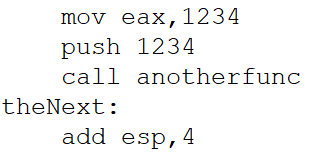
\includegraphics[width=5cm]{call.png}
	\bicaption{call指令示例汇编代码}{Call instruction sample assembly code}
	\label{call1}
\end{figure}

除第三条指令外,其他指令都是在一个栈层次上进行,不需要更换栈,但是第三条指令“CALL anotherfunc”是对其他函数的调用,它的栈帧会改变,所以必须将控制权交给其他代码。

汇编语言中,CALL指令先把当前执行指令的下一条指令压入栈中,然后再跳转到目标函数的首地址处,代码如图\ref{a}所示,将控制权交给其他代码之后必须再跳回虚拟机中,所以使用代码如图\ref{b}所示,这是返回虚拟的一段代码,NextCode代表THEnext之后代码的字节码。只需要将thenext的地址修改为nextVM的地址,便可以再次模拟一个CALL指令,vcall指令的伪代码如图\ref{c}所示。


\begin{figure}[htbp]
	\centering
	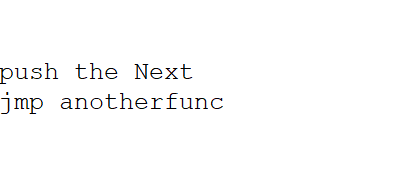
\includegraphics[width=6cm]{a.png}
	\bicaption{目标函数的首地址}{The starting address of the target function}
	\label{a}
\end{figure}

\begin{figure}[htbp]
	\centering
	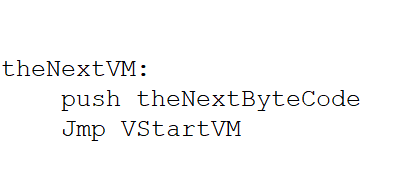
\includegraphics[width=6cm]{b.png}
	\bicaption{跳回虚拟机代码}{Jump back to the virtual machine code}
	\label{b}
\end{figure}

\begin{figure}[htbp]
	\centering
	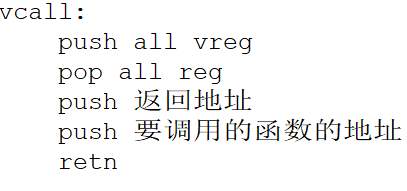
\includegraphics[width=6cm]{c.png}
	\bicaption{vcall指令的伪代码}{The pseudocode for the VCall directive}
	\label{c}
\end{figure}



\section{本章小结}
本章采用虚拟机保护的方法对Windows下可执行文件进行了保护,并提出一种多样化Handler设计思路,实现了该方法,对转移指令、算术指令、CALL指令进行了多样化设计,由于X86架构和汇编语言的特性,指令本身的实现不是唯一的,将Handler分为辅助Handler和普通Handler,以低耦合的特点设计了汇编语言和字节码之间的转换协议,本章的试验将会在后文进行详细描述。